\documentclass[a4paper,german,12pt,smallheadings]{scrartcl}
\usepackage[T1]{fontenc}
\usepackage[utf8]{inputenc}
\usepackage{babel}
\usepackage{geometry}
\usepackage{pdfpages}
\usepackage{tikz}
\usepackage{wrapfig}
\usepackage[fleqn]{amsmath}
\usepackage{amssymb}
\usepackage{float}
\usepackage{enumerate}
\usepackage{listings} % Source code
\usepackage{lscape} % landscape
\usepackage{commath} % http://tex.stackexchange.com/questions/14821/whats-the-proper-way-to-typeset-a-differential-operator
\usepackage{cancel}
\usepackage[fleqn]{mathtools}
% Number only referenced equations
%\mathtoolsset{showonlyrefs}

%\usepackage{wrapfig}
\usepackage{siunitx}
\sisetup{separate-uncertainty=true,locale=DE}

% New command for color underlining
\usepackage{xcolor}
\newcommand\invisiblesection[1]{%
    \refstepcounter{section}%
      \addcontentsline{toc}{section}{\protect\numberline{\thesection}#1}%
        \sectionmark{#1}}
\newsavebox\MBox
\newcommand\colul[2][red]{{\sbox\MBox{$#2$}%
  \rlap{\usebox\MBox}\color{#1}\rule[-1.2\dp\MBox]{\wd\MBox}{0.5pt}}}

\restylefloat{table}
\geometry{a4paper, top=15mm, left=20mm, right=10mm, bottom=20mm, headsep=10mm, footskip=12mm}
\linespread{1.5}
\setlength\parindent{0pt}
\DeclareMathOperator{\Tr}{Tr}
\DeclareMathOperator{\Var}{Var}
\begin{document}

\begin{titlepage}
\newcommand{\HRule}{\rule{\linewidth}{0.5mm}}

\begin{center}
  \textsc{\Large Physikalisches Grundpraktkum 1}
  \HRule\\[0.4 cm]
  {\huge \bfseries Gleichmäßig beschleunigte Drehbewegungen}
  \HRule\\[0.4 cm]

  \begin{minipage}{0.65\textwidth}
  \begin{flushleft}
    Markus Fenske \texttt{<iblue@zedat.fu-berlin.de>} \\
    Paul Rahmann \texttt{<paulrahmann@zedat.fu-berlin.de>}
  \end{flushleft}
  \end{minipage}
  \hfill
  \begin{minipage}{0.30\textwidth}
  \begin{flushright}
    Tutor: Christian Hindermann \\
    Versuchstag: 6. Juni 2014
  \end{flushright}
  \end{minipage}

  \vspace{1cm}

  \tableofcontents


  %{\large \today}
  \vfill
\end{center}
\newpage

\end{titlepage}

\allowdisplaybreaks % Seitenumbrüche in Formeln erlauben
\begin{center}
\bfseries % Fettdruck einschalten
\sffamily % Serifenlose Schrift
\vspace{-40pt}
Physikalisches Grundpraktikum 2, Wintersemester 2014/2015

Markus Fenske \texttt{<iblue@zedat.fu-berlin.de>}

Alexandra Krause \texttt{<alexandra.krause2@gmail.com>}

Mikroskop, Tutor: Kevin Madsen
\vspace{-10pt}
\end{center}

\section{Physikalische Grundlagen}

Das menschliche Auge ist in der Lage Gegenstände ab einer Größe von $0{,}02
\operatorname{mm}$ zu betrachten. Um kleinere Gegenstände wahrzunehmen, werden
optische Hilfsmittel wie Lupe oder Mikroskop benötigt. Diese sollen im
folgenden untersucht werden.

\subsection{Geometrische Optik}

Die Physik kennt viele verschiedene Beschreibungen der elektromagnetischen
Wellen. Für den Spezialfall des Lichtes in der Optik besonders geeignet ist die
\textit{Geometrische Optik}. Dabei wird die Wellen- und Teilchennatur des
Lichtes vernachlässigt und vereinfachend angenommen, das Licht bestünde aus
Lichtstrahlen, die sich geradlinig fortbewegen und ihre Richtung nur an
jeweiligen Brechkanten gemäß des Snelliusschen Brechnungsgesetzes ändern (siehe
vorheriger Versuch).

\subsection{Dünne Linsen}

Besonders wichtig für diesen Versuch ist dabei die Beschreibung von
Sammellinsen. Sammellinsen sind in erster Näherung Glaskörper in der Form der
Schnittmenge zweier gleich großer Vollkugeln. Interessant ist, in welcher Art
sich nun Lichtstrahlen durch Sammellinsen bewegen. Man stellt fest, dass für
den Spezialfall, dass die Linse klein gegenüber dem Radius der begrenzenden
Vollkugeln sind, dass es drei Arten von Strahlen gibt, die sich gegenüber den
anderen auszeichnen:

\begin{itemize}
  \item Der \textit{Mittelpunktstrahl} durchläuft die Linse ohne durch
    Brechnung abgelenkt zu werden.
  \item Der \textit{Parallelstrahl} trifft parallel zur optischen Achse (also
    der Achse durch den Mittelpunkt der beiden gedachten Vollkugeln) auf die
    Linse. Er wird immer derart gebrochen, dass er durch einen Punkt geht, den
    wir im folgenden als \textit{Brennpunkt} $F$ bezeichnen wollen.
  \item Da es sich um eine bijektive Abbildung handelt, wird jeder Strahl der
    durch den Brennpunkt geht wieder zum Parallelstrahl. Diesen nennen wir
    \textit{Brennpunktstrahl}.
\end{itemize}

% FIXME: Abbildung Strahlengang in TikZ

Die folgende Zeichnung gibt unter Verwendung dieser Definitionen den
Strahlengang durch eine dünne Linse an.


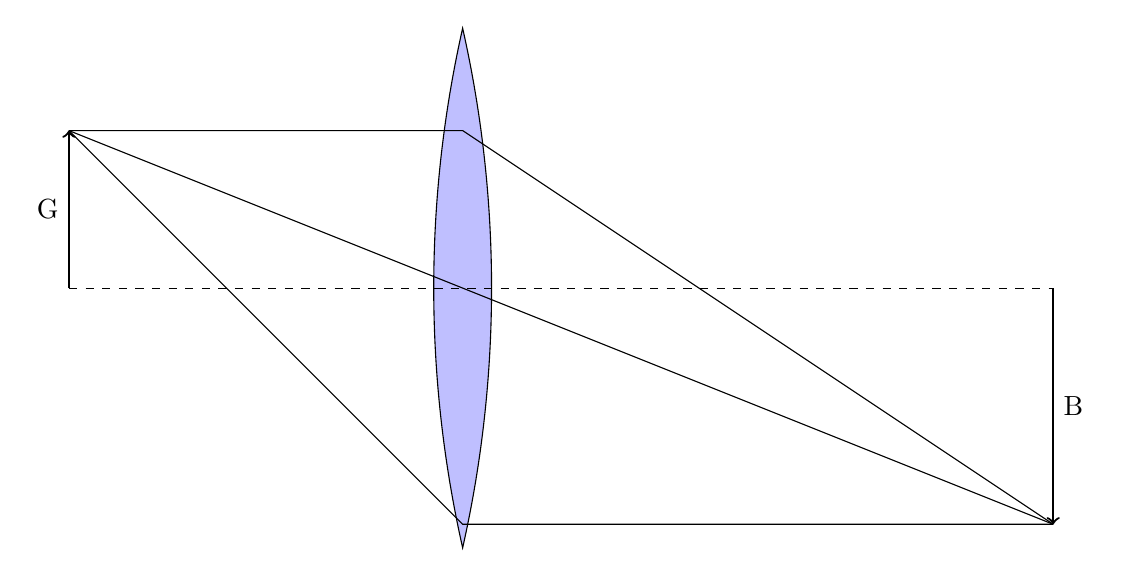
\begin{tikzpicture}
  \pgfmathsetmacro{\lensRadius}{15}
  \pgfmathsetmacro{\lensHeight}{3.3}
  \pgfmathsetmacro{\startAngle}{asin(\lensHeight/\lensRadius)}
  \pgfmathsetmacro{\focalLength}{3}
  \pgfmathsetmacro{\objectDistance}{5}
  \pgfmathsetmacro{\objectHeight}{2}
  \pgfmathsetmacro{\pictureDistance}{1/((1/\focalLength)-(1/\objectDistance))}
  \pgfmathsetmacro{\pictureHeight}{\pictureDistance/\objectDistance*\objectHeight}

  % Linse
  \draw [fill=blue!25]  (0,\lensHeight)
  arc[start angle=180-\startAngle,delta angle=2*\startAngle,radius=\lensRadius]
  arc[start angle=-\startAngle,delta angle=2*\startAngle,radius=\lensRadius]
   -- cycle;

  % Gegenstand
  \draw[thick,->] (-\objectDistance,0) -- node[left] {G} (-\objectDistance,\objectHeight);

  % Bild
  \draw[thick,->] (\pictureDistance,0) -- node[right] {B} (\pictureDistance,-\pictureHeight);

  % Mittelpunktstrahl
  \draw (-\objectDistance,\objectHeight) -- (\pictureDistance,-\pictureHeight);

  % Parallelstrahl
  \draw (-\objectDistance,\objectHeight) -- (0,\objectHeight) -- (\pictureDistance,-\pictureHeight);

  % Brennpunktstrahl
  \draw (-\objectDistance,\objectHeight) -- (0,-\pictureHeight) -- (\pictureDistance,-\pictureHeight);

  % Optische Achse
  \draw[dashed] (-\objectDistance,0) -- (\pictureDistance,0);
\end{tikzpicture}



% FIXME: Abbildung
Die Dreiecke bestehend aus den Strecken $G$, $g$ und dem halben
Mittelpunktstrahl und aus $B$, $b$ und dem halben Mittelpunktstrahl sind
ähnlich, denn sie stimmen in allen Winkeln überein (rechter Winkel zwischen $G$
und $g$ sowie $B$ und $b$ und Wechselwinkel am Mittelpunktstrahl). Somit müssen
die Streckenverhältnisse gleich sein. Wir definieren darüber den
Abbildungsmaßstab $\beta$.

\begin{equation}
  \beta = \frac{B}{G} = \frac{b}{g}
  \label{eq:beta}
\end{equation}

Auf der Seite des Bildes ergibt wird ein Dreieck gebildet aus der der Strecke
$f$, der Gegenstandshöhe $G$ in der Linsenebene und dem halben
Brennpunktstrahl. Das Dreieck aus $B$, $b-f$ und der anderen Hälfte des
Brennpunktstrahls ist dazu aus den selben Gründen wie oben ähnlich. Somit gilt

\begin{equation}
  \frac{B}{G} = \frac{b-f}{f}
\end{equation}

Zusammengesetzt ergibt sich
\begin{equation}
  \frac{b}{g} = \frac{b-f}{f}
  \label{eq:inter}
\end{equation}

Durch Division durch $b$ und Addition von $\frac{1}{b}$ erhält man die
Abbildungsgleichung

\begin{equation}
  \frac{1}{f} = \frac{1}{b} + \frac{1}{g}
\end{equation}

% Aufgabe 2

Für einen festen Abstand $e$ zwischen Gegenstand und Bild gilt $e = g+b$.

% http://www.wolframalpha.com/input/?i=solve+1%2Ff+%3D+1%2Fg+%2B+1%2F%28e-g%29+for+g
Durch Einsetzen in die Linsengleichung ergeben sich also nur zwei Lösungen für
ein scharfes Bild. % FIXME: Herleitung (Umstellen, PQ-Formel)

\begin{equation}
  g = \pm \frac{1}{2} \del{\sqrt{e^2 - 4ef} + e}
\end{equation}

Dabei handelt es sich einmal um eine Vergrößerung ($\beta > 1$) und einmal um
eine Verkleinerung ($\beta < 1$). % FIXME: Warum? beta = (e-g)/g für beide
% Lösungen ausrechnen!

% Aufgabe 3
% FIXME: Einführung dicke Linsen
Die geometrischen Überlegungen gelten genauso für dicke Linsen, denn entfernt
man die Hauptebenen, ergeben sich die selben geometrischen Zusammenhänge.
Problematisch ist nur, dass sich aufgrund des unbekannten Hauptebenenabstands
die Gegenstands- und die Bildweite nicht mehr bestimmen lassen. Der Brennwert
muss sich also aus einem anderen Zusammenhang ergeben. Messbar sind $g-b$ und
$\beta$, so dass daraus der Brennwert berechnet werden muss.

Durch Einsetzen von \ref{eq:beta} in \ref{eq:inter} erhalten wir

\begin{equation}
  \beta = \frac{b-f}{f}
\end{equation}

Umgestellt nach $f$:
\begin{equation}
  f = \frac{b}{\beta + 1}
\end{equation}

Durch Erweitern mit $\beta - 1$:
\begin{equation}
  f = \frac{b(\beta - 1)}{1-\beta^2}
\end{equation}

Durch Erweitern mit $\frac{1}{\beta} = \frac{g}{b}$:

\begin{equation}
  f = \frac{g - b}{\frac{1}{\beta} - \beta}
\end{equation}

Somit ist die Brennweite nur durch $g-b$ und $\beta$ ausgedrückt.

Aus $e = g + i + b$ erhalten wir

\begin{align*}
  i &= e - (g+b) \\
    &= e - (g-b) \frac{g+b}{g-b} \\
    &= e - (g-b) \frac{(g+b)\beta}{(g-b)\beta} \\
    &= e - (g-b) \frac{b + \beta b}{b - \beta b} \\
    &= e - (g-b) \frac{\beta + 1}{\beta - 1}
\end{align*}

% Aufgabe 4: Zeug malen (Aus Skript übernehmen?)

% Aufgabe 5:
% FIXME: Einleitung Mikroskop
Analog zu oben kann man sich den Vergrößerungsfaktor des Objektivs geometrisch
überlegen.

% FIXME: Hier Grafik mit Hervorhebung der beiden Dreiecke.
Auf der Bildseite des Objektivs bildet die Strecke $f_1$ zusammen mit $G$ und
der Hälfte des Mittelpunktstrahls ein Dreieck das ähnlich ist zu dem Dreieck
aus $t$, $B$ und der anderen Hälfte des Mittelpunktstrahls. Somit ist

\begin{equation}
  \beta_\text{ob} = \frac{B}{G} = \frac{t}{f_1}
\end{equation}

Durch die Definition $\Gamma_\text{ob} := \beta_\text{ob}$ des
Vergrößerungsfaktors ist also

\begin{equation}
  \Gamma_\text{ob} = \frac{t}{f_1}
\end{equation}

% FIXME: Herleitung Okular. Akkomodation??? Unklar. Zusammenstümpern!


\end{document}
